\section{Questão 151 Laranja Ledor - Interpretação de gráficos}

Na anestesia peridural, como a usada nos partos, o médico anestesista precisa introduzir uma agulha nas costas do paciente, que atravessará várias camadas de tecido até chegar a uma região estreita, chamada espaço epidural, que envolve a medula espinhal. A agulha é usada para injetar um líquido anestésico, e a força que deve ser aplicada à agulha para fazê-la  avançar através dos tecidos é variável.

A figura é um gráfico do módulo F da força (em newton) em função do deslocamento x da ponta da agulha (em milímetro) durante uma anestesia peridural típica. 

\noindent \textbf{Descrição da figura:} A figura mostra um gráfico em um plano cartesiano. O eixo x representa o deslocamento da ponta da agulha, em milímetro, e o eixo y representa o módulo da força, em Newton. O gráfico é representado por uma linha poligonal com oito segmentos, 

\noindent Segmento AB: do ponto A(0 ; 0) ao ponto B(8 ; 12).

\noindent Segmento BC: do ponto B(8 ; 12) ao ponto C(12 ; 6).

\noindent Segmento CD: do ponto C(12 ; 6) ao ponto D(18 ; 8).

\noindent Segmento DE: do ponto D(18 ; 8) ao ponto E(20 ; 7).

\noindent Segmento EF: do ponto E(20 ; 7) ao ponto F(26 ; 7).

\noindent Segmento FG: do ponto F(26 ; 7) ao ponto G(28 ; 12).

\noindent Segmento GH: do ponto G(28 ; 12) ao ponto H(30 ; 12).

\noindent Segmento HI: do ponto H(30 ; 12) ao ponto I(32 ; 3).


Considere que a velocidade de penetração da agulha deva ser a mesma durante a aplicação da anestesia e que a força aplicada à agulha pelo médico anestesista em cada ponto deve ser proporcional à resistência naquele ponto.

Com base nas informações apresentadas, a maior resistência à força aplicada observa-se ao longo do segmento

\noindent (A) AB.

\noindent (B) FG.

\noindent (C) EF.

\noindent (D) GH.

\noindent (E) HI.


\textbf{Resolução}

A figura descrita pode ser desenhada da seguinte forma:

\noindent \resizebox{\linewidth}{!}{
    \begin{tikzpicture}[scale=.5,y=1cm, x=.7cm,font=\sffamily]
        %axis
        \draw [->] (0,0) -- coordinate (x axis mid) (32,0);
        \draw [->] (0,0) -- coordinate (y axis mid) (0,14);
        %ticks
        \foreach \x in {0,5,...,32}
        \draw (\x,1pt) -- (\x,-3pt) node[anchor=north] {\x};
        \foreach \y in {0,...,14}
        \draw (1pt,\y) -- (-3pt,\y)  node[anchor=east] {\y}; 
        %labels      
        \node[below=0.8cm] at (x axis mid) {x = deslocamento da agulha [mm]};
        \node[rotate=90, above left=0.8cm and .8cm] at (y axis mid) {y = módulo da força [N]};
        
        %plots
        \node[label={-45:{A( 0 ; 1 )}},circle,fill,inner sep=2pt] at (0,0) (A) {};
        \node[label={90:{B( 8 ; 12 )}},circle,fill,inner sep=2pt] at (8,12) (B) {};
        \node[label={-90:{C( 12 ; 6 )}},circle,fill,inner sep=2pt] at (12, 6) (C) {};
        \node[label={90:{D( 18 ; 8 )}},circle,fill,inner sep=2pt] at (18, 8) (D) {};
        \node[label={-120:{E( 20 ; 7 )}},circle,fill,inner sep=2pt] at (20, 7) (E) {};
        \node[label={120:{F( 26 ; 7 )}},circle,fill,inner sep=2pt] at (26, 7) (F) {};
        \node[label={120:{G( 28 ; 12 )}},circle,fill,inner sep=2pt] at (28, 12) (G) {};
        \node[label={46:{H( 28 ; 12 )}},circle,fill,inner sep=2pt] at (30, 12) (H) {};
        \node[label={0:{I( 32 ; 3 )}},circle,fill,inner sep=2pt] at (32, 3) (I) {};

        
        \draw [ultra thick	] (A) -- (B) -- (C) -- (D) -- (E) -- (F) -- (G) -- (H) -- (I) ;
    \end{tikzpicture}
}

Vemos claramente que estamos falando que a resistência e a força aplicada são proporcionais, ou seja, o segmento com maior parte dela na parte superior do gráfico, o que acontece em 2 treços, no ponto B e no segmento GH, que é nossa resposta procurada, o que corresponde ao gabarito (D)

\textbf{Observação}

Na prova azul da segunda aplicação a questão 142 traz o gráfico conforme a prova oficial:

\begin{figure}[H]
    \centering
    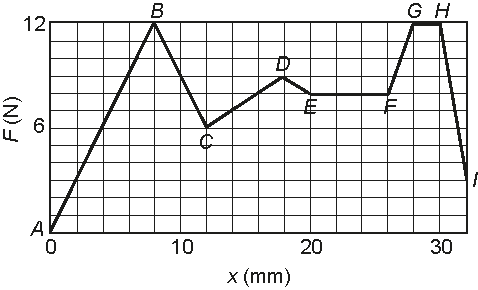
\includegraphics[width=0.99\linewidth]{Q142-R}
    \caption{}
    \label{fig:q142-r}
\end{figure}


\begin{center}
    \href{https://youtu.be/}{
        \qrcode{https://youtu.be/}
    }\\
    Resolução: \url{https://youtu.be/}
\end{center}
